\documentclass[../mainfile.tex]{subfiles}


\begin{document}
\section{The Dirichlet Problem via Brownian Motion}
Before we discuss the connection between Brownian motion and the Dirichlet problem, we will briefly talk about coupling techniques which will come in useful. 
\subsection{Coupling}
\subsubsection{Coupling in $1$D}
Suppose that one considers $x$ and $\hat{x}$ in $\mathbb{R}$, such that $x \neq \hat{x}$. It is our goal to define on the same probability space two Brownian motions $B$ and $\hat{B}$ started from $x$ and $\hat{x}$ respectively in such a way that \textit{"after they meet"}, they \textit{"stick together"}. Obviously these two Brownian motions would not be independent of one another. We discuss two ideas:
\subsubsection{First idea: $B$ and $\hat{B}$ move independently, until they meet}
Let $B$ and $\tilde{B}$ be two independent Brownian motions, started from $x$ respectively $\hat{x}$ and define $T= \inf \{ t >0 : B_t = \tilde{B}_t \}$. We then define $\hat{B}$ by:
\begin{align*}
\hat{B}_t := \begin{cases} \tilde{B}_t, & t \leq T \\
B_t, & t >T \end{cases}
\end{align*}
one can then check that the law of $(\hat{B}_t)_{t \geq 0}$ is still that of a Brownian motion. 
\begin{figure}[hbtp]
\centering
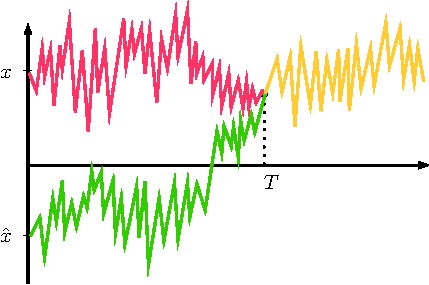
\includegraphics[scale=.8]{coupling1.pdf}
\caption{We see the sample of a Brownian motion $B$ (red + orange) and the sample of $\tilde{B}$ independent BM (green) and the new BM $\hat{B}$ (green + orange).}
\end{figure}
\newpage
\subsubsection{Second idea: Mirror coupling}
Let assume that $x=-\hat{x}>0$ (for convenience purposes, otherwise we shift everything by $(x+\hat{x})/2)$. Let us sample the Brownian motion $(B_t)_{t \geq 0}$ started from $x$ and then define $T= \inf \{ t >0 : B_t =0 \}$. We then define $\hat{B}$ by 
\begin{align*}
\hat{B}_t := \begin{cases} -B_t , & t \leq T \\ B_t, & t > T \end{cases}
\end{align*}
it is then again easy to check that $\hat{B}$ is a Brownian motion. $\hat{B}$ is called the mirror coupling of $B$ started from $-x$. 
\begin{figure}[hbtp]
\centering
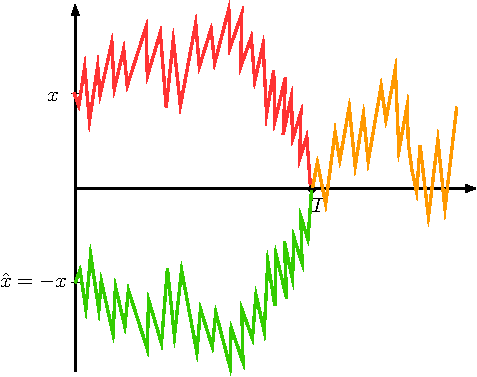
\includegraphics[scale=.9]{mirrorcoupling.pdf}
\caption{Mirror coupling: We see the sample of the Brownian motion $B$ (red + orange) and it's mirror $-B_t$ (green) and the BM $\hat{B}$ (green + orange).}
\end{figure}
\subsubsection{Mirror coupling in $\mathbb{R}^d$}
Let us consider $x \neq 0$ in $\mathbb{R}^d $ and $\hat{x}=-x$. Let $\mathcal{H}$ be the hyperlane of points that are equidistant to $x$ and $\hat{x}$ (i.e. $\mathcal{H}$ is the median hyperplane between $x$ and $-x$). Let now $(B_t)_{t \geq 0}$ be a Brownian motion started from $x$. \\\\
 Let $T = \inf \{ t >0 : B_t \in \mathcal{H}\}$ and let us denote by $\sigma$ the symmetry with respect to the hyperplane $\mathcal{H}$. We then define $\hat{B}$ as
 \begin{align*}
 \hat{B}_t := \begin{cases} \sigma(B_t), & t \leq T \\
 B_t, & t > T \end{cases}
 \end{align*}
 \newpage

\begin{figure}[hbtp]
\centering
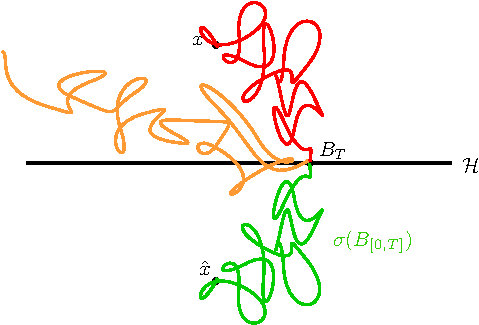
\includegraphics[scale=.9]{mirrorcoupd.pdf}
\caption{Mirror coupling in $\mathbb{R}^d$: A BM in $\mathbb{R}^d$ started from $x$ (red + orange) and its mirror (w.r.t. $\mathcal{H})$ started $\hat{x}$ (green) and it's mirror coupling $\hat{B}$ which is a BM started from $\hat{x}$ (green + orange).}
\end{figure}
\subsection{Towards the Dirichlet Problem}
We use our multidimensional ideas to develop a more substantial consequence.
\begin{defn} We say that a bounded open subset $D$ of $\mathbb{R}^d$ satisfies property $(\mathcal{P})$ if, for every $x \in \partial D$, there exists $r>0$ and a sequence $x_n \to x$ such that for all $n$ we have
\begin{align*}
\mathcal{B}(x_n,r \|x_n-x\|) \cap D = \emptyset. 
\end{align*}
\end{defn}
\begin{figure}[hbtp]
\centering
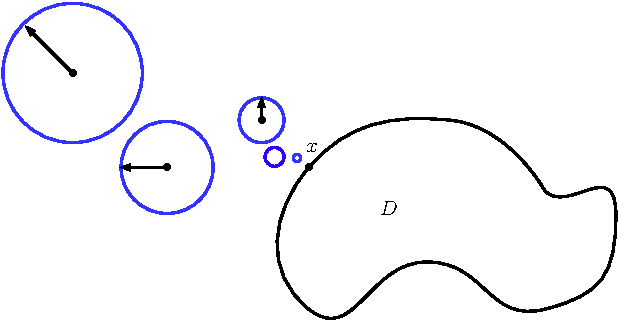
\includegraphics[scale=.8]{propp.pdf}
\caption{A depiction of property ($\mathcal{P})$. }
\end{figure}
\begin{rem} Obviously $(\mathcal{P})$ is satisfied as soon as for each $x \in \partial D$, there exists an open cone $C$ with apex at $x$ such that $C \cap \overline{D}= \emptyset$. This is often referred to as the \textit{outside cone condition}. 
\end{rem}
\newpage
Suppose that $D$ is a bounded open subset of $\mathbb{R}^d$. Suppose that we are given a continuous, real-valued function $f$ that is defined on $\partial D$.
\\\\
 We are now going to define a (very nice) function $U$ on $\overline{D}$ using Brownian motion. For each given $x \in \overline{D}$, we consider a Brownian motion $(B_t)_{t \geq 0}$ started from $x$. Let $T$ be the first time where $B$ hits the boundary of $D$, i.e. \begin{align*}
T = \inf \{ t >0 : B_t \in \partial D \},
\end{align*}
(note that $T$ is finite because $D$ is bounded). We then define for all $x \in \overline{D}$ 
\begin{align*}
U(x):= \mathbb{E}_x (f ( B_T)). 
\end{align*}
\begin{figure}[hbtp]
\centering
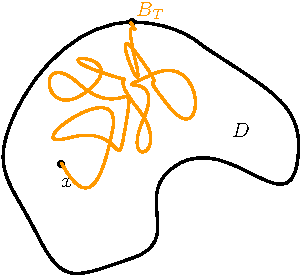
\includegraphics[scale=.9]{funcU.pdf}
\caption{We start a BM at $x \in \overline{D}$ and let it evolve until it hits the boundary of $D$ (equivalently: until it escapes the set $D$).}
\end{figure}
\begin{prop} \label{propfuncU} When $D$ is a bounded open subset of $\mathbb{R}^d$, and $f$ is a continuous, real-valued function defined on $\partial D$, then the function $U$ satisfies the following properties:
\begin{itemize}
\item $U$ is continuous in $D$.
\item $U$ is equal to $f$ on $\partial D$.
\item $U$ satisfies the "mean-value property" in $D$: For all $x \in D$ and for all \\ $r<d(x, \partial D)$, the mean value of $U$ on the sphere of radius $r$ around $x$ is equal to $U(x)$, or in a formula:
\begin{align*}
U(x)= \int_{S(x,r)} U(z)d \sigma_{x,r}(z),
\end{align*}
where $\sigma_{x,r}$ is the (unique) uniform probability measure on the sphere $S(x,r)$ of radius $r$ around $x$. 
\end{itemize}
\end{prop}
\newpage
\begin{rem} Notice that we do not state here that the function $U$ is continuous at the boundary points of $D$. However, we will later on give a condition such that this will be the case. 
\end{rem}
\begin{proof}
We first give a rough sketch before we provide more detail. The second statement is obvious, if we have $x \in \partial D$, then obviously $T=0$ and thus $B_T=B_0=x$, in particular we have $U(x)=\mathbb{E}_x(f(x))=f(x)$. The first statement will be derived using mirror coupling. The final statement will follow from the strong Markov property at the hitting time of the sphere $S(x,r)$ by $B$. 
\\\\
\textbf{Continuity:} Let us fix $x \in D$ and let $r_0=d(x, \partial D)$. Choose $y$ with $d(x,y) < r_0/8$. Set $x_0=(x+y)/2$, then $x_0$ is equidistant from $x$ and $y$ and we can consider the hyperplane $\mathcal{H}$ through $x_0$. We now consider the two coupled Brownian motions:
\begin{align*}
\begin{cases} B, \text{ Brownian motion started from $x$} \\
B', \text{ "mirror coupled BM" started from $y$}
\end{cases}
\end{align*}
We then have for fixed $r_1$, the probability that $B$ and $B'$ do not couple before $B$ hits $\mathcal{B}(x_0,r_1)$ goes to $0$ as $d(x,y) \to 0$. 

\begin{figure}[hbtp]
\centering
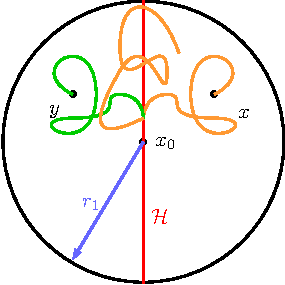
\includegraphics[scale=1]{couplingproof.pdf}
\caption{For a fixed $r_1$, the probability that the BM (orange) does not couple with its coupled mirror $B'$ (green) before $B$ exits $\mathcal{B}(x_0,r_1)$ goes to $0$ when the distance between $x,y$ is small. In Particular $B_T=B_T'$ with high probability when $y$ is close to $x$.}
\end{figure}
\begin{align*}
|\mathbb{E}(f(B_T)-f(B_T'))| \leq \mathbb{E}(|f(B_T)-f(B_T')|) \\
\leq 2 \|f\|_\infty \mathbb{P}(B \text{ and } B' \text{ do not couple before reaching } \mathcal{B}(x_0,r_1)) \overset{y \to x}\longrightarrow 0
\end{align*}
We conclude that $|U(y)-U(x)| \to 0$ as $y \to x$. 
\newpage
\textbf{Mean-value property:} We take $x \in D$ and let $r < d(x, \partial D)$. We consider a Brownian motion $B$ started from $x$, and we let $\tau$ be the first time at which it hits the sphere $S(x,r)=\partial \mathcal{B}(x,r)$ around $x$ of radius $r$, i.e. 
\begin{align*}
\tau = \inf \{ t>0 : d(B_t,x)=r \}. 
\end{align*}
We have 
\begin{align*}
U(x)=\mathbb{E}_x(\mathbb{E}(f(B_T) \mid \mathcal{F}_\tau))
\end{align*}
and we can apply the strong Markov property at time $\tau$, it states that conditionally on $\mathcal{F}_\tau$, the process $(B_{\tau+t)})_{t \geq 0}$ is again  a Brownian motion started from $\tau$, hence we have
\begin{align*}
\mathbb{E}(f(B_T) \mid \mathcal{F}_\tau ) = \mathbb{E}_{B_\tau}(f(B_T))=U(B_\tau),
\end{align*}
but we know that the law of $B_\tau$ is uniformly distributed on the sphere $\partial \mathcal{B}(x,r)$ which then proves the claim. Recall that a Brownian motion (in distribution) is invariant under rotations (in fact, by the law of Isotropy it is invariant under linear isometries). The only probability measure on the sphere $S(x,r)$ that is invariant under rotations is the uniform measure (see for instance Exercise 5.1).
\begin{figure}[hbtp]
\centering
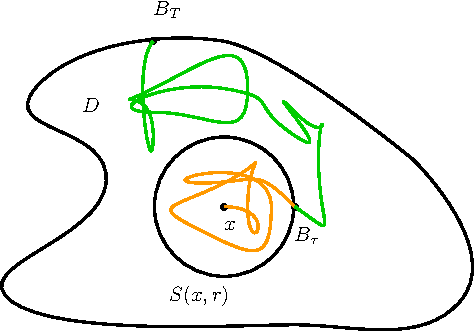
\includegraphics[scale=1]{meanvalueprop.pdf}
\caption{Conditionally on $\mathcal{F}_\tau$, we observe another Brownian motion $(B_{\tau+t})_{t \geq 0}$ started from $\tau$ (and independent of $\mathcal{F}_\tau)$} 
\end{figure}
\\
\end{proof}
\newpage
Let us now give a condition on $D$ that ensures that $U$ will also be continuous at boundary points (i.e. on $\partial D)$. 
\begin{defn} We say that $x \in \partial D$ is a regular boundary point of $D$, if when one considers a Brownian motion $B$ started from $x$, then almost surely 
\begin{align*}
\inf \{ t > 0: B_t \notin D \} =0,
\end{align*}
i.e. a BM started from $x \in \partial D$ exits immediately $\overline{D}$. We say that $D$ has a regular boundary for Brownian motion (or in short, a regular boundary) if every boundary point is regular. 
\end{defn}
\begin{rem} We know that the exterior cone condition implies property $(\mathcal{P})$, but then it also has a regular boundary (because we know that almost surely, for all $\epsilon >0$ there exists $t \in (0, \epsilon)$ such that $B_t \in \mathcal{C})$. 
\end{rem}
\begin{prop} \label{propUcontboundary} Let us consider $D$ and $U$ just as in Proposition \ref{propfuncU}. If we also assume that $D$ has a regular boundary for Brownian motion, then the function $U$ is continuous on $\overline{D}$. 
\end{prop}
The idea in order to prove this Proposition goes as follows: Let $x_0 \in \partial D$ be a regular boundary point and $y \in D$ such that $d(y,x)$ is very small, then with high probability, a Brownian motion started from $y$ will exit $D$ near $x_0$, so in particular with high probability the value of $f$ at the exit point is close to $f(x_0)$. This is made more precisely by the following Lemma:
\begin{lem} Let $x_0$ be a regular boundary point of the bounded domain $D$. For all $\epsilon >$ and $\delta >0$, there exists $r>0$, such that for all $x \in \mathcal{B}(x_0,r) \cap D,$ we have 
\begin{align*}
\mathbb{P}_x(d(B_t,x_0) > \delta) < \epsilon. 
\end{align*}
\end{lem}
\begin{figure}[hbtp]
\centering
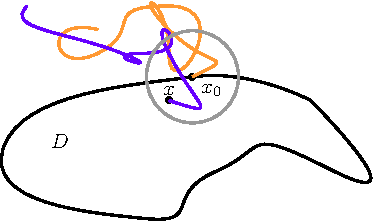
\includegraphics[scale=.8]{lemmaexittime.pdf}
\caption{$x_0$ is a regular boundary point (BM exits $D$ immediately started from there), if we choose $x$ according to the Lemma above and start a BM from there, then with high probability we exit $D$ near $x_0$.} 
\end{figure}
\newpage
\begin{proof}[Proof of Proposition]
Let $x_0 \in \partial D$. Our goal is to prove that the function $U$ is continuous at $x_0$. We notice that $U(x_0)=f(x_0)$ by definition. We know that $f$ is continuous at $x_0$ and $|f|$ is bounded by $M:=\|f\|_\infty < \infty$. Thus by the continuity of $f$ at $x_0$ we have for all $ \epsilon >0$, the existence of $\delta >0$ such that for all $y \in \mathcal{B}(x_0, \delta) \cap \partial D : |f(y)-f(x_0)| < \epsilon$. (*)
\\\\
For this choice of $\epsilon$ and $\delta$ we use the previous Lemma. It gives us the existence of a radius $r>0$ such that for all $x \in D \cap \mathcal{B}(x_0,r)$, when $B$ is a Brownian motion started from $x$, with probability at least $1- \epsilon$ (very high), one has $d(B_T,x_0) < \delta$, hence we have $B_T \in \mathcal{B}(x_0, \delta) \cap \partial D$ which immediately implies (making use of (*)) that $|f(x_0)-f(B_T)| < \epsilon$. \\\\
In the event that $d(B_T,x_0) \geq \delta$ (which happens only with very small probability $\leq \epsilon$), we anyway have that $|f(x_0)-f(B_T)| \leq 2M$. We can then conclude that
\begin{align*}
|U(x)-f(x_0)| \leq \mathbb{E}_x(|f(B_T)-f(x_0)|) \leq \epsilon \overbrace{\mathbb{P}_x(d(B_T,x_0) < \delta)}^{\leq 1} +  2M \mathbb{P}_x(d(B_T,x_0) \geq \delta) \\ \leq \epsilon + 2 M \underbrace{\mathbb{P}_x(d(B_T,x_0) \geq \delta)}_{\leq \epsilon} \leq \epsilon (1 + 2 M),
\end{align*}
where we again used the previous Lemma. This proves that $U$ is continuous at $x_0$. 
\end{proof}
\newpage
\subsection{Harmonic Functions, Brownian Motion and the Dirichlet Problem}
Throughout this section, $\Omega$ will denote any (not necessarily bounded) open subset of $\mathbb{R}^d$. There are two natural definitions of harmonic functions: Via the mean value property, or via the Laplacian. As we shall see, these two definitions are in fact equivalent. 
\begin{defn} We say that the function $h: \Omega \to \mathbb{R}$ is harmonic in $\Omega$, if it is continuous in $\Omega$ and if it satisfies the following mean-value property: For each $x \in \Omega$ and each $r < d(x, \partial \Omega)$, 
\begin{align*}
h(x) = \int_{S(x,r)} h(z) d \sigma_{x,r}(z),
\end{align*}
where $\sigma_{x,r}$ is the uniform probability measure on the sphere $S(x,r)= \partial \mathcal{B}(x,r)$. 
\end{defn}
\begin{rem} 
\begin{enumerate}
\item We can read the mean-value property as $h(x)=$ mean-value of $h$ on $S(x,r)= \partial \mathcal{B}(x,r)$. 
\item We shall later prove that harmonic functions are in fact necessarily smooth. 
\end{enumerate}
\end{rem}
We suppose from now on that $D$ denotes a \textit{bounded} open subset of $\mathbb{R}^d$. Suppose we are given a continuous function $f: \partial D \to \mathbb{R}$. Given that $\partial D$ is compact, such a function $f$ is necessarily bounded. We then define:
\begin{defn}A function $h: \overline{D} \to \mathbb{R}$ is said to be a solution to the Dirichlet problem in $D$ with boundary values $f$ if it satisfies:
\begin{itemize}
\item $h$ is harmonic in $D$.
\item $h$ is continuous in $\overline{D}$ and $h=f$ on $\partial D$. 
\end{itemize}
\end{defn}
\begin{figure}[hbtp]
\centering
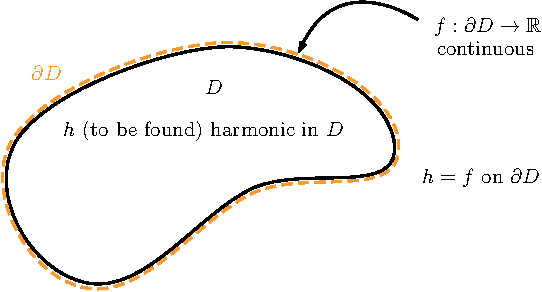
\includegraphics[scale=.86]{dirichletprob.pdf}
\end{figure}
\newpage
Here is a simple classical result that we will use
\begin{lem}[Maximum principle I] Suppose that $H$ is a continuous function on $\overline{D}$ that is harmonic in $D$. Then $\sup_{\overline{D}} H= \max_{\partial D} H$, i.e. such a function takes its maximum value on the boundary of $D$. 
\end{lem}
\begin{cor} There exists at most one solution to the Dirichlet problem. 
\end{cor}
\begin{proof}
If we have two solutions $h_1$ and $h_2$, then $H:=h_1-h_2$ and $-H$ are harmonic in $D$, continuous in $\overline{D}$ and equal to $0$ on $\partial D$ (because they both satisfy the same boundary condition). Applying the maximum principle I to $H$ and $-H$, 
\begin{align*}
\begin{cases} \max_{\overline{D}}H= \max_{\partial D} H= \max_{ \partial D} (h_1-h_2) =0 \\ \max_{\overline{D}} (h_2-h_1)=0
\end{cases}
\end{align*}
from which we conclude that $H=0$ on $\overline{D}$ and thus, i.e. $h_1=h_2$ on $\overline{D}$. 
\end{proof}
At the end of the previous section, we have used Brownian to construct a concrete candidate for the solution of the Dirichlet problem, and we did in fact show that under some conditions on $D$ (on its boundary), it was a solution to the Dirichlet problem.
\\\\ Let us repeat the construction here: We suppose that $D$ and $f$ are given as introduced in this section. Then for each $x \in \overline{D}$, we define a Brownian motion $B$ started from $x$ under the probability measure $\mathbb{P}_x$ (we write $\mathbb{E}_x$ for the expectation with respect to this probability measure). We also let $T$ be the first time at which the Brownian motion $B$ hits $\partial D$. Then we define for each $x \in \overline{D}$, 
\begin{align*}
U(x):= \mathbb{E}_x(f(B_T)).
\end{align*}
If we now combine Proposition \ref{propfuncU}, Proposition \ref{propUcontboundary} together with the uniqueness statement of the above corollary we obtain
\begin{thm} If all the boundary points of the bounded domain $D$ are regular, then there exists a unique solution to the Dirichlet problem, and this solution is equal to the function $U$. 
\end{thm}
So, it remains to see what can happen when some boundary points of $D$ are not regular. We will state (and prove) a general fact that is valid for any bounded domain $D$. Notice that in the next proposition we don't impose any conditions on the boundary of $D$ (i.e. regularity).
\newpage
\begin{prop} If the solution to the Dirichlet problem in bounded $D$ with boundary values $f$ exists, then it is necessarily equal to the function $U$. 
\end{prop}
As an important consequence to the above Proposition (and the previous Theorem) there are just two options:
\begin{itemize}
 \item Either $U$ is a solution to the Dirichlet problem and then a solution exists and it is unique, 
 \item or $U$ is not a solution to the Dirichlet problem and then it means that there is no solution to the Dirichlet problem at all (because if it would exist, it would have to be equal to $U$ according to the above Proposition).
\end{itemize}
  Proposition \ref{propUcontboundary} shows that the only thing that can prevent $U$ from being a solution to the Dirichlet problem is the possible lack of continuity of $U$ at the boundary points. As we will see a little bit later, it can indeed happen that $U$ has discontinuities at non-regular boundary points. 
\begin{proof}[Proof of Proposition] Suppose that $h$ is a solution to the Dirichlet problem in $D$ with boundary values $f$. Let us fix $x \in D$ and we want to show that $h(x)=U(x)$. Let $B$ be a Brownian motion started from $x$, and we define iteratively the following stopping times: $T_0=0$ and for each $n \geq 0$, we set $r_n=d(B_{T_n}, \partial D)$ and 
\begin{align*}
T_{n+1} = \inf \{ t > T_n : d(B_t, B_{T_n}) = r_n/2 \}. 
\end{align*}
We notice that $r_0=d(B_0, \partial D)=d(x, \partial D)$ and $T_1 = \inf \{ t >0: d(B_t,x) = r_0/2\}$ is the first time we hit the sphere $S(x,r_0/2)$. 
\begin{figure}[hbtp]
\centering
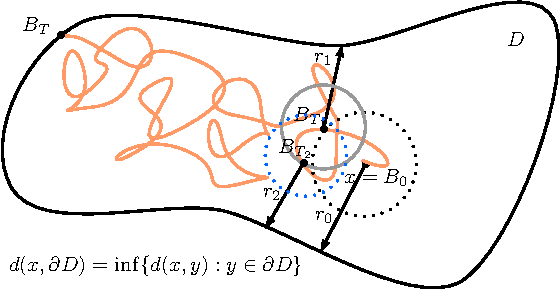
\includegraphics[scale=1.2]{proofwendi.pdf}
\caption{The sequence of the stopping times $T_n$.}
\end{figure}
\newpage
Since we know that almost surely, $B$ is continuous and will exit $D$ almost surely, we can deduce iteratively that $T_n < T < \infty$ almost surely and that $r_n \geq r_0/2^n >0$. 
 The continuity of Brownian motion also implies that $T_n$ is increasing, thus it converges almost surely to some $T'$ with $T' \leq T$. To see that $T' \geq T$ assume for contradiction that $r':= d(B_{T'}, \partial D) >0$, then for $n \in \mathbb{N}$ sufficiently large enough we get that 
 \begin{align*}
d(B_{T_{n+1}}, B_{T_n})= \frac{r_n}{2} > \frac{r'}{4}>0.
 \end{align*}
But the continuity of $B$ ensures that $B_{T_n}$ converges to $B_{T'}$ and thus the above is a contradiction, we conclude that $r'= d(B_{T'}, \partial D)=0$, i.e. $T' \in \partial D$ and since by definition $T$ is the first hitting time of the boundary of $D$ we conclude that $T' \geq T$. \\
\\
The continuity of $h$ and $B$ now ensures that,
\begin{align*}
h(B_{T_n}) \overset{a.s.}\longrightarrow h(B_T)=f(B_T).
\end{align*}
On the other hand, using the strong Markov property at time $T_n$ and the harmonicity of $h$ we get that for all $n \in \mathbb{N}_{ \geq 1}$, almost surely 
\begin{align*}
h(x)= \mathbb{E}_x(h(B_{T_n})).
\end{align*}
Indeed, for $n=1$ we have by the harmonicity of $h$ and by the definition of $T_1$ as the hitting time of sphere with radius $r_0/2$ around $x$ that
\begin{align*}
h(x)= \text{mean value of $h$ on } S(x,r_0/2)= \mathbb{E}_x(h(B_{T_1}))
\end{align*}
Assume now that we have $h(x)= \mathbb{E}_x(h(B_{T_n}))$. We then have by the strong Markov property,
\begin{align*}
\mathbb{E}_x(h(B_{T_{n+1}})) = \mathbb{E}_x( \mathbb{E}( h(B_{T_{n+1}}) \mid \mathcal{F}_{T_n})) \overset{1)}= \mathbb{E}_x( \mathbb{E}_{B_{T_n}}( h(B_{T_{n+1}})))& \overset{2)}= \mathbb{E}_x(h(B_{T_n})) \\ &=h(x),
\end{align*}
where in 1) we used the strong Markov property at time $T_n$ and in 2) the harmonicity of $h$. Hence, by dominated convergence ($h$ is bounded on $\overline{D}$, because $\overline{D}$ is compact and $h$ is continuous on $\overline{D}$) we get that
\begin{align*}
h(x)= \mathbb{E}_x(h(B_{T_n})) \to \mathbb{E}_x(f(B_T))=U(x)
\end{align*}
which concludes the proof.
\end{proof}
\begin{rem} \
\begin{enumerate}
\item In class Prof. Werner mentioned that he likes this proof.
\end{enumerate}

\end{rem}
\newpage
\subsubsection{Harmonic Functions}
Let us come back to the other possible definition of harmonicity:
\begin{prop} Let $\Omega$ be an open set in $\mathbb{R}^d$. A function $h : \Omega \to \mathbb{R}$ is harmonic in $\Omega$ if and only if $h$ is $C^2$ in $\Omega$ and $\Delta h=0$ in $\Omega$. Moreover, a harmonic function is necessarily smooth (i.e. $C^\infty$). 
\end{prop}
\begin{rem} Hence, the Dirichlet problem (as we defined it) is equivalent to the more standard  phrasing: Find a function $h$ that is continuous in $\overline{D}$, equal to $f$ on $\partial D$, is $C^2$ in $D$ and such that $\Delta h=0$ in $D$. 
\end{rem}
\begin{proof}[Proof very sketchy] "$\Longrightarrow$" is a convolution argument which shows that $h \in C^\infty$, in particular in $C^2$ and we can use the Taylor expansion and the harmonicity of $h$ to derive $\Delta h=0$. 
\\
"$\Longleftarrow$" Uses the Maximum principle II below: For $r<d(x, \Omega)$ we work on $D= \mathcal{B}(x,r)$ (this domain satisfies property ($\mathcal{P})$) and we know that the D.P. with boundary values given by $H$ has a unique solution given by $U$. But then $U$ is $C^\infty$ and its Laplacian vanishes in $D$, by 2MP $U=H$ in $D$. But then $U(x)=H(x)$ is the mean value of $H$ on $\mathcal{S}(x,r)$.

\end{proof}
\begin{lem}[Maximum principle II] If $h$ is a $C^2$ function in $D$ that is continuous on $\overline{D}$ such that $\Delta h \geq 0$ in $D$, then 
\begin{align*}
\max_{\overline{D}} h = \max_{\partial D} h. 
\end{align*}
\end{lem}
\subsubsection{Some consequences for multidimensional Brownian motion}
In the previous sections, we have used Brownian motion in order to construct the unique possible solution to the Dirichlet problem. In this section, we will use their identification in terms of Brownian motion expectations, in order to deduce some explicit formulas for Brownian motion hitting probabilities. 
\\\\
Let us first look at the case $d=2$. Let $B$ be a Brownian motion in dimension $2$ started from $x$. Let $H(x)= \log ( |x|)$ be defined on $\mathbb{R}^2 \setminus \{0\}$, we can then easily see that $H$ is harmonic because its Laplacian is $0$. This means, by the uniqueness of the solution to the Dirichlet problem, that for every bounded domain $D$ with regular boundary and such that $\overline{D} \subset \mathbb{R}^2 \setminus \{0\}$ we have 
\begin{align*}
\log(|x|)= \mathbb{E}_x( \log |B_T|), \text{ for all } x \in D,
\end{align*}
where $T$ denotes the exit time of $B$ from $D$. 
\\\\
Let us now apply this to a more concrete example.
\newpage
\begin{exmp} Let us fix $0<r<R$ and take $D= \mathcal{B}(0,R) \setminus \mathcal{B}(0,r)$, then $D$ has a regular boundary because it satisfies property ($\mathcal{P})$. Let us start a Brownian motion inside $D \subset \mathbb{R}^2 \setminus \{0\}$ and consider the hitting times
\begin{align*}
T_r&= \inf \{ t>0 : |B_t| =r \} \\
T_R& = \inf \{ t >0 : |B_t|=R\} \\
T&= T_r \wedge T_R \text{ is the exit time of }D. 
\end{align*}
We know that for all $x \in D$ we have 
\begin{align*}
\log(|x|)= \mathbb{E}_x( \log |B_T|).
\end{align*}
Thus we obtain 
\begin{align*}
\log(|x|) &= \mathbb{E}_x( \log |B_T| 1_{T_r < T_R}) + \mathbb{E}_x( \log |B_T| 1_{T_R < T_r})  \\
&= \mathbb{E}_x( \log|B_{T_r}| 1_{T_r < T_R}) + \mathbb{E}_x( \log( |B_{T_R}| 1_{T_R < T_r}) \\
&= \log|r| \mathbb{P}_x( T_r < T_R) + \log|R| \mathbb{P}_x(T_R < T_r)  \\
& = \log(r) (1- \mathbb{P}_x(T_R < T_r)) + \log(R) \mathbb{P}_x ( T_R < T_r).
\end{align*}
The above yields:
\begin{align*}
\mathbb{P}_x( T_R < T_r) = \frac{\log(|x|)- \log(r)}{\log(R)- \log(r)} \tag{*}
\end{align*}
If we now let $R \to \infty$, then we get almost surely that $T_R \to \infty$ (by the continuity of Brownian motion) and thus 
\begin{align*}
\mathbb{P}_x(T_r = \infty) = \lim_{R \to \infty} \mathbb{P}_x( T_r > T_R)=0
\end{align*}
for some fixed $r>0$ and $x$ with $|x|>r$. Thus we have shown:
\begin{prop} Almost surely, for all fixed $r>0$, a two dimensional Brownian motion started from $x$ with $|x|>r$ will visit $\mathcal{B}(0,r)$. 
\end{prop}
From this proposition we can immediately get:
\begin{thm} For two-dimensional Brownian motion, the set $\{B_t: t \geq 0\}$ is almost surely dense in the plane, i.e. $\overline{B[0, \infty)}= \mathbb{R}^2$.
\end{thm}
\begin{proof}
The previous proposition equivalently states that for $B$ Brownian motion in $d=2$ started from $0$ we have for all $x \in \mathbb{R}^2 \setminus \{0\}$ and for all $r<d(x,0)$ almost surely that $B$ will visit the disk $\mathcal{D}(x,r)$. This statement is true almost surely simultaneously  for all $x \in \mathbb{Q}^2 \setminus \{0\}$ and for all $r \in \mathbb{Q}_+$, but the set of such rational couples $(x,r)$ (simultaneously) is countable. 
\end{proof}
\newpage
If we now fix $x$ and $R$ in (*) and let instead $r \to 0$, we have $T_r \to 0$ (continuity of Brownian motion), we then easily see that
\begin{align*}
\mathbb{P}_x(B \text{ hits the point $0$ before }T_R)= \lim_{r \to 0} \mathbb{P}_x (T_r < T_R) \\ = 1 - \lim_{r \to 0} \mathbb{P}_x(T_R < T_r)=1-1=0.
\end{align*}
We have thus proven
\begin{prop}
Almost surely, a two-dimensional Brownian motion that starts away from the origin will never visit the origin. 
\end{prop}
\end{exmp}
Let us now consider the $3$ dimensional case. In this case we know that $H(x)=1/\|x\|$ defined on $\mathbb{R}^3 \setminus \{0\}$ is Harmonic because its Laplacian is $0$.
\begin{exmp} Let us again fix $0<r<R$, $D, T_r,T_R,T$ all as in the previous example. Let $B$ be a $3$ dimensional Brownian motion started inside $D \subset \mathbb{R}^3 \setminus \{0\}$. We then have again for all $x \in D$ that 
\begin{align*}
|x|^{-1} = \mathbb{E}_x( 1/|B_T|)=  r^{-1} \mathbb{P}_x(T_r < T_R) + R^{-1}(1 - \mathbb{P}_x(T_r < T_R))
\end{align*}
which implies that 
\begin{align*}
\mathbb{P}_x(T_r < T_R) = \frac{|x|^{-1}-R^{-1}}{r^{-1}-R^{-1}}.
\end{align*}
If we let $R \to \infty$ we get that $T_R \to \infty$ (because BM is continuous) and thus \begin{align*}
0< \mathbb{P}_x(T_r < \infty) = \frac{r}{|x|}<1 \tag{**}
\end{align*}
where $|x| >r$ (because we start $B$ in $D$). If we now let $r \to 0$ in (**) we obtain \begin{align*}
\mathbb{P}_x(B \text{ hits the point $0$ before it escapes to $\infty$}) = \lim_{r \to 0} \mathbb{P}_x( T_r < \infty) = 0
\end{align*}
This (and the fact that when $d \geq 3$, the first three coordinates of a $d$-dimensional Brownian motion form a $3$-dimensional Brownian motion) in turn implies that:
\begin{prop}\label{propescinfty} If $B$ is a Brownian motion in dimension $d \geq 3$, then almost surely it escapes to infinity, in particular $\|B_t\| \to \infty$ as $t \to \infty$. 
\end{prop}
\end{exmp}
\begin{rem}Recall that for a simple random walk in $\mathbb{Z}^d$, it is recurrent when $d=2$ and transient when $d \geq 3$. So, we see that there is a little difference in the way in which two-dimensional Brownian motion is recurrent (it almost surely visits all open sets infinitely often) compared to the recurrence of simple random walk (that almost surely visits every point infinitely often). 
\end{rem}
\newpage
\subsection{Dirichlet Problem on non-regular boundary points}
Let us now briefly come back to the discussion about the existence of bounded domains $D$ for which the solution to the Dirichlet problem might not exist. 
\begin{exmp} Arguably the simplest example, is the case of the planar domain $D= \mathcal{B}(0,1) \setminus \{0\}$, i.e. the unit disk minus its center. Then, it is clear that the origin is not a regular boundary point. Indeed, we know that a Brownian motion started from the origin will almost surely never return to the origin. So if we define
\begin{align*}
f(x) = \begin{cases} f(x)=1, & \text{on } \partial B(0,1) \\
 f(0)=0 \end{cases}
\end{align*}
then $f: \partial D \to \mathbb{R}$ is continuous on the boundary of $D$ (i.e. on $\partial \mathcal{B}(0,1) \cup \{0\}$). 
\\\\
We then have for all $x \in D$ 
\begin{align*}
U(x)= \mathbb{E}_x(f(B_T))=1,
\end{align*}
because Brownian motion started from $x \in D$ will almost surely exit $D$ on the unit circle. But  \begin{align*}
U(x) \overset{x \to 0}\longrightarrow 1 \neq U(0) =f(0)=0.
\end{align*}
Hence $U$ is not continuous at $x=0$ and consequently $0$ is not a regular boundary point. So, there is no solution to the Dirichlet problem for this choice of $D$ and $f$. 
\end{exmp}
\begin{figure}[hbtp]
\centering
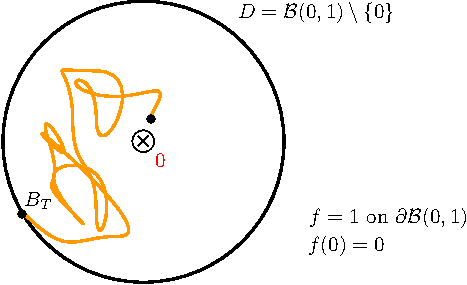
\includegraphics[scale=.9]{nonregularboundary.pdf}
\caption{The above example suits to give a non regular boundary point $x=0$.}
\end{figure}
\begin{rem} We highlight that the most important argument used in this example is that a $2$-dimensional Brownian motion started away from the origin will never visit the origin again. 
\end{rem}
\newpage
\begin{exmp} Another example is the following three-dimensional counterpart to the previous example. Let us consider the unit ball $\mathcal{B}(0,1)$ in $\mathbb{R}^3$. Let $u=(0,0,1) \in \mathbb{R}^3$ be the north pole of the unit sphere and let us denote by $I$ the segment that joins the origin to the point $u$, i.e. $I=[0,u]$. We then choose $D = \mathcal{B}(0,1) \setminus I$.  \\
\\
We then obtain a continuous function $f: \partial D= \mathcal{S}(0,1) \cup I \to \mathbb{R}$ by setting 
\begin{align*}
f(x) = \begin{cases} f(x)=1,  &\text{ on } \mathcal{S}(0,1) \\ f(x)=0, & \text{ on } I  \end{cases}
\end{align*} 
We know that almost surely a two-diemsnional Brownian never hits the origin at positive times. Hence, the Brownian motion $B$ started in $x \in D$ will not hit $I$ at positive times (because the projection of such a BM onto the horizontal plane is a $2d$ BM that will a.s. never visit the origin at positive times). \\
\\
Thus we have $B_T \in \mathcal{S}(0,1)$ whenever $B_0 \notin I$. Thus we obtain that every $x \in [0,u)$ (notice right open, $u$ is regular because of the outside cone condition) is not a regular boundary point. Indeed we have for all $x \in D$ 
\begin{align*}
U(x)= \mathbb{E}_x(f(B_T))=1
\end{align*}
in particular we obtain that 
\begin{align*}
U(x) \overset{x \to 0}\longrightarrow 1 \neq U(0)= f(0)=0
\end{align*}
This shows that for all $x \in [0,u)$ that $U$ is not continuous at such a $x$. In particular all said $x$ are not regular boundary points for $D$ and there exists no solution to the Dirichlet problem for said choice of $D$ and $f$. 
\end{exmp}
\begin{figure}[hbtp]
\centering
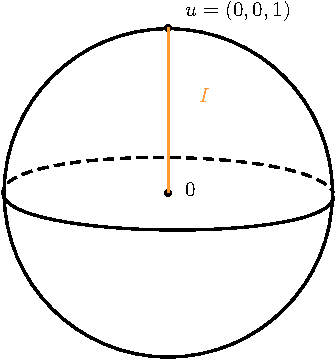
\includegraphics[scale=.86]{3dnonregular.pdf}
\end{figure}
\newpage
\begin{exmp} One may wonder whether the result we obtained from the previous example is only due to the fact that $I$ is "one-dimensional" and has no interior. Here is another, more involved example, that shows that this is not the case. \\
Recall that a Brownian motion $B$ started from $0$ in $\mathbb{R}^3$ does almost never visit the line that goes through the origin and $u=(0,0,1)$ at positive times and that  $\|B_t\| \to \infty$ (which implies that the set of points visited by $B$ is closed).
\\\\
Let $(r_n)_{n \in \mathbb{N}}$ be a sequence of radii such that $r_n \to 0$ as $n \to \infty$. Let $c_n$ be the closed segment of radius $r_n$ between the points $(0,0,2^{-n})$ and $(0,0,2^{-(n+1)})$. 
\begin{figure}[hbtp]
\centering
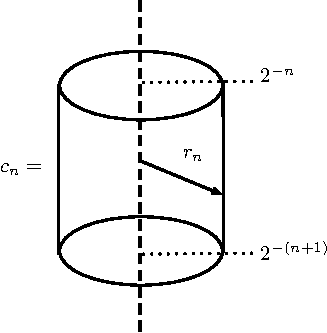
\includegraphics[scale=.9]{ceen.pdf}
\caption{The $c_n$ as depicted as above are the "drills" we're going to apply to sphere,  see figure further below. }
\end{figure} \\
We then define: $D= \mathcal{B}(0,1) \setminus \Big( \overline{\bigcup_{n \geq 0 } c_n} \Big)$
\begin{figure}[hbtp]
\centering
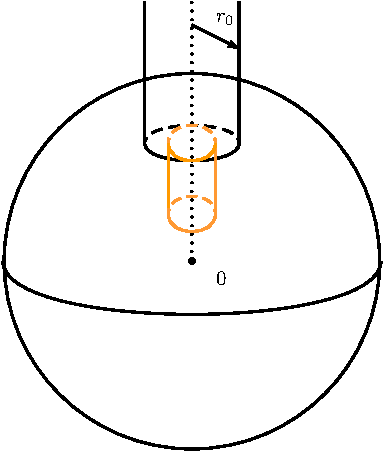
\includegraphics[scale=.70]{drilling.pdf}
\caption{We apply gradually finer and finer drills ($c_n$ above) to $\mathcal{B}(0,1)$ until we reach $0$.}
\end{figure}
\newpage
Let us define $I=[u/2,u] \subset \mathbb{R}^3$. This is a compact set and thus the distance between the closed set $\{B_t, t \geq 0\}$ is strictly positive. I.e. if we take a Brownian motion $B$ started from $0$ then almost surely $d(\{B_t, t \geq 0\}, I) >0$ which gives that
\begin{align*}
 \mathbb{P}(d( \{B_t, t \geq 0\}, I) <r ) \to 0 \text{ as } r \to 0.
\end{align*}
Let us choose $r_n'$ such that \begin{align*}
\mathbb{P}(d(B,I) < r_n') \leq \frac{1}{2^{n+2}}.
\end{align*}
By scaling invariance of Brownian motion we obtain that 
\begin{align*}
\mathbb{P}(d(B,2^{-n}I) < 2^{-n} r_n') = \mathbb{P}(d(B,I) < r_n') \leq \frac{1}{2^{n+2}},
\end{align*}
therefore we get
\begin{align*}
\mathbb{P}( \exists n \geq 0 : d(B,2^{-n}I) < 2^{-n}r_n') \leq \sum_{n \geq 0} \frac{1}{2^{n+2}}= \frac{1}{2}
\end{align*}
and consequently 
\begin{align*}
\mathbb{P}\left(B \text{ never intersects } \bigcup_{n \geq 0 } \{ z : d(z,2^{-n}I)< 2^{-n}r_n'\} \right) \geq \frac{1}{2}.
\end{align*}
So if we define $r_n:= 2^{-n}r_n'$, then the above yields that a Brownian motion started from $0$ has a probability of at least $1/2$ to exit $D$ through $\partial B(0,1)$. In other words $0$ is not a regular boundary point of $D$. \\
\\
We can then define the function $f(x)= \| x \|$ on $\partial D$, and we can show that there exists a sequence $x_n$ in $D$ such that $x_n \to 0$ but $U(x_n) \not\to 0 = U(0)=f(0)=0$. (Will be discussed in more detail in the exercise sheets).  
\end{exmp}
\newpage
\subsubsection{Some final remarks on the Dirichlet problem}
We want to give some concluding remarks on the Dirichlet problem. In particular one should pay attention to the second remark presented here, where we discuss how odd things can happen once unbounded domains $D$ are considered (we can for instance lose uniqueness of solutions).
\begin{rem} It is worthwhile to stress that while for most domains (for instance bounded domains that satisfy the exterior cone condition), it is possible to prove existence and uniqueness of the solution to the Dirichlet problem without the use of probability theory and Brownian motion. \\
\\
However, Brownian motion appears to be the right tool when one tries to describe exactly which bounded domains have the property that for all continuous functions $f$, the solution to the Dirichlet problem exists. Indeed, the previous ideas (theorems and examples) suggest that a \textbf{necessary and sufficient condition} is exactly that all boundary points are \textbf{regular}. This will be derived in the exercise sheets. 
\end{rem}
\begin{rem} When the domain $D$ is not bounded and $d  \geq 3$, one has to be careful because it could happen that with positive probability, a Brownian motion started in $D$ does in fact stay in $D$ forever.
\\
\\
For instance, if one considers $D= \mathbb{R}^d \setminus \overline{\mathcal{B}(0,1)}$, we have seen that with positive probability, a Brownian motion started form $x \in D$ does wander away to infinity without hitting $\mathcal{S}(0,1)$ (see (**) before Proposition \ref{propescinfty}), i.e. the exit time $T$ of $D$ is infinite with positive probability. 
\\
\\
So we see that for all $c \in \mathbb{R}$,  the functions 
\begin{align*}
H(x):= c \mathbb{P}_x(T = \infty)
\end{align*}
are all harmonic in $D$, continuous on $\overline{D}$ and equal to $0$ on $\mathcal{S}(0,1)$. In particular the solution to the Dirichlet problem in $D$ for $f=0$ is therefore not unique. 
\end{rem}
\newpage
\subsection{Story time} 
In this section we briefly discuss some further features of Brownian motion. The content of this section is more for \textit{scientific culture} and should be viewed more as a story telling session without full proofs, where only the main ideas of the proofs will be hinted at. 
\subsubsection{Polar sets for planar Brownian motion}
Suppose we consider a compact set $K$ in the plane and a planar Brownian motion started at $x \notin K$. We can ask which sets $K$ do have the property that there will almost surely never be hit by $B$. 
\begin{defn} If $\mathbb{P}( \exists t \geq 0 : B_t \in K)=0$, then we say that $K$ is a polar set for our planar Brownian motion. 
\end{defn}
We want to study which compact sets in $\mathbb{R}^2$ a Brownian motion does not hit. So what do we know?
\begin{enumerate}
\item If $K$ is a singleton, then it is polar (because planar Brownian motion almost surely does not visit a given point). 
\begin{enumerate}
\item Consequently, if $K$ is countable, then it is polar (because the union of countably many events with probability $0$ has probability $0$). 
\end{enumerate}
\item If $K$ is a line segment $[a,b]$, then it is not polar (i.e. $\mathbb{P}(B$ hits $K)=1$).
\item If $\overset{\circ}K \neq \emptyset$, then $K$ is not polar. 
\end{enumerate}
The question we are going to address here is what happens to sets $K$ such as the classical Cantor set, which is a subset of an interval with length zero. Recall briefly the construction of the Cantor set:\\
\\
We start with $I_0=[0,1] \subset \mathbb{C} \sim \mathbb{R}^2$ (unit length). We then define iteratively \begin{align*}
I_1&= [0,1/3] \cup [2/3,1]
\end{align*}
$I_2$ is obtained by cutting out the (open) middle third of each of the $2$ closed intervals of $I_1$.\\
$I_{k+1}$ is obtained by cutting out the (open) middle third of each of the $2^k$ closed intervals (of length $3^{-k}$) that $I_k$ is the union of. It is then well known that $K:= \cap_{k}I_k$ is a compact set, with zero length, but it is uncountable and has the same cardinality as $\mathbb{R}$. 
\newpage
So we ask us the question, does Brownian motion hit the Cantor set $K$?
\begin{prop} The Cantor set $K$ is not a polar set for planar Brownian motion (i.e. $B$ hits $K$ almost surely). 
\end{prop}
This shows that while two-dimensional Brownian motion does not hit points, it nevertheless hits fairly small sets. 
\subsubsection{Two cousins of the Dirichlet problem}
We are now going to quickly discuss how problems related to the Dirichlet problem can also be interpreted and solved using Brownian motion. 
\\\\
Just as in the Dirichlet problem,  we are going to suppose that $D$ is an open bounded subset of $\mathbb{R}^d$ with a regular boundary (all boundary points are regular boundary points), and we are given a real valued continuous function $f$ defined on $\partial D$. Let us also assume that we are given a constant $\alpha \geq 0$. 
\\
\\
\textbf{Goal}: Find a function $h$ such that:
\begin{itemize}
\item $h$ is $C^2$ in $D$ and in $D$ satisfies $\Delta h = \alpha h$.
\item $h$ is continuous on $\overline{D}$ and $h=f$ on $\partial D$. 
\end{itemize}
\begin{rem} We notice that in the special case of $\alpha =0$ this is just classical Dirichlet problem that we have already studied. 
\end{rem}
\begin{prop}The solution to this new problem exists and is unique,  and it is equal to the function 
\begin{align*}
U(x) = \mathbb{E}_x(f(B_T)e^{ - \alpha T}), \text{ for all } x \in \overline{D}.
\end{align*}
\end{prop}
\begin{rem} We notice again that for $\alpha=0$ we just obtain again the classical solution to the Dirichlet problem.
\end{rem}
We will prove this result later with the help of stochastic calculus.
\\\\
Yet another variant of the Dirichlet problem is the following: We still consider a bounded domain $D$ in $\mathbb{R}^d$, and we are given a constant $\beta$. This time we look for a solution to the following problem: Find a function $H$ that is continuous in $\overline{D}$, equal to $0$ on $\partial D$, that is $C^2$ in $D$ and that satisfies $\Delta H = - 2 \beta$ in $D.$
\begin{prop} There exists a unique solution to this problem, and it is given by the function
\begin{align*}
U(x)= \mathbb{E}_x( \beta T), \text{ for all } x \in \overline{D}. 
\end{align*}
\end{prop}
\end{document}
